\documentclass{article}
\usepackage{amsmath, amssymb, textcomp}
\usepackage{graphicx}
\usepackage{cite}
\usepackage[hidelinks]{hyperref}
\usepackage[section]{placeins}

\newcommand{\Part}[3][ ]{\ensuremath{\frac{\partial^{#1} #2}{{\partial #3}^{#1}}}}
\newcommand{\Dif}[3][ ]{\ensuremath{\frac{d^{#1} #2}{{d #3}^{#1}}}}
\renewcommand{\O}[1]{\ensuremath{\mathcal{O}\left(#1\right)}}
\renewcommand{\vec}{\bold}

\begin{document}
\title{Plasma Analysis}
\author{Tobias de Jong \& David Kok}
\date{\today}
\maketitle

\section{Introduction}
{\bf Fysische achtergrond, motivatie voor numeriek. Bonuspunten voor gebruik van het woord Topologisch }
We will use CUDA to efficiently calculate the topological properties of magnetic field lines as generated by Chris Smiet's simulations.\cite{PhysRevLett.115.095001}\\
Smiet's work concentrates on plasma's in which the field lines have a non-trivial topological order, such as interlocking rings. Since field lines can not cross, this topological order enhances the stability of the plasma.

The simulations we used as starting data for the analysis in this report do MHD calculations in order to calculate the evolution through time of the plasma, starting out with two or more interlocked rings, evolving into nested tori.
Of this tori we want to calculate properties, foremost the winding number.

To implement the code we were inspired by Marek Fiser.\footnote{\url{http://www.marekfiser.com/Projects/Real-time-visualization-of-3D-vector-field-with-CUDA}} He uses Runge-Kutta integration to visualize (air) flows around a Delta wing, but the idea of integration of a vector field is the same.

\section{Theory and Methods}
\subsection{Theory}
We want to calculate properties of the magnetic field by using field lines associated to the field. In order to do this we need to calculate (finite segments of) field lines. To do this it is enough to note that field lines are the solutions $\vec x(s)$ to the following ordinary differential equation:
\[\Dif{\vec x}{s} = \vec B(\vec x),\]
where $s$ is the parametrization variable.\\
An interesting observation made by \textbf{insertrefhere} is that in an ideal plasma the total helicity of the field, defined through the volume integral:
\[
\text{Helicity} = \int\vec{A}\cdot\vec{B}\ d\vec{x} = \int\vec{A}\cdot (\nabla\times\vec{A})d\vec{x}
\]
is conserved. Therefore the initial value of this integral restricts the possible long-term dynamics of a plasma. In particular we are working with a dataset of highly helical initial data, in which case the field lines will align themselves along the surfaces of nested tori. A line on the surface of a torus can be associated with a winding number, which is the ratio of the winding along the toroidal axis (denoted with $\alpha$) and the winding along the poloidal axis (in our code denoted with $\beta$). To calculate a field line and its winding numbers we will use numerical integration as described in more detail below.


\subsection{Methods}
The goal of our project is to determine topological properties of a pre-computed magnetic field from a magnetohydrodinamical simulation.\\
Our code is split into two main segments. Firstly we numerically integrate the magnetic field to obtain (a numerical approximation of) a field line in the plasma. Secondly we compute several properties of the magnetic field using this field line, such as the length of the line (which estimates the average field strength), the center of the line (estimating the origin of the torus on which it lies) and its winding number, i.e. its contribution to the total helicity of the magnetic field.\\
Both steps can be parallelized heavily. To parallelize the numerical integration of the magnetic field we simply consider more than one field line at a time. In the second step we not only consider multiple field lines at once, but also parallelize the computation of the aforementioned parameters per field line.\\


\section{Numerical theory}
{\bf complexiteit in termen van relevante parameters}
\subsection{Vector field representation}
To represent the vector field $\vec{B}: \mathbb{R}^3 \to \mathbb{R}^3$ in a computer we need to discretize this field. This is done by defining a grid in space and saving the components of the field at each grid point. Note that we are interested in the field lines for fixed moments in time, so all our analysis will not concern the time evolution of the plasma. There are two ways to save all the components: either seperate the components and save a three-dimensional array for each component of the vector field (three $N\times N\times N$ arrays), or save one large array of which each component contains the whole vector at the corresponding gridpoint (one $N\times N\times N$ array of $3D$ vectors).

Since numerical integration algorithms will use all the components of the field at a point at the same time we use the second method. %Or do we? Ik weet eigenlijk niet hoe een 3D texture van binnen werkt...
This choice of representation is both physically intuitive as well as efficient, since it will improve cache coherency and therefore access times.

\subsubsection{Interpolation}
In order to accurately integrate we need very accurate estimates of the original vectorfield at arbitrary locations. It is unfeasable to have such a fine discretization that we have a value for each location of interest. We therefore want to interpolate the vector field to get a good approximation of the value of the vector field at an arbitrary location. The simplest method for interpolation is linear interpolation, for 3D data known as trilinear interpolation.

Interpolation of two- and even three-dimensional data is used in graphics processing in order to map images onto three-dimensional objects. In graphics processing this is known as texturing. Because this problem is very important in graphics processing modern GPU's have efficient texturing units, performing trilinear interpolation in hardware.

Using CUDA enables us to use this hardware accelerated interpolation by storing our vector field data as a texture. Since every RK4-step needs at least 4 vector field fetches this acceleration significantly speeds up the numerical integration. %alhoewel we dit natuurlijk niet gemeten hebben.

\subsection{Runge-Kutta method}
For line integration the fourth order Runge-Kutta method (RK4) was used.  This method is known as a good allround integration method. Compared to standard Forward Euler, RK4 uses four values of the magnetic field to calculate the next point on the field line. This increase in calculation time per step is compensated by a vastly reduced error per step, allowing for a much larger step size $\Delta s$, since RK4 is a fourth order method with total accumulated error $\O{\Delta s^4}$.

\subsection{Algorithm}
To calculate the winding number of a field line passing through a certain starting point we first use RK4 to integrate a large length of field line from the magnetic field data. This process is inherently sequential. Since the interpolation is hardware optimized we are memory access bound in this part of the algorithm, which we have verified by using the NVIDIA profiler. Thus there was nothing to be gained from parallelizing the integration further than one-thread-per-field-line.

To compute the winding number of a field line we need to convert to a toroidal coordinate system. Since not all tori of interest are perfectly aligned this means we first have to find the position and orientation of the torus of interest before we can calculate any other relevant parameters.

By averaging the coordinates over a whole field line we find (a good approximation of) the origin of our torus. This summation can be done efficiently in parallel as a reduction. For implementation we implemented most of the methods described by Harris et al.~\cite{harris2007optimizing}.

Next we need to calculate the orientation of the torus, in particular the normal to the surface plane of the torus. We can find this normal by taking the outer product of the direction of a field line (the $\vec{B}$-field) at a point and the location vector of that point. We perform this local calculation for each point on our field line and implement a similar parallel reduction as before to find the orientation of our torus.

The last part of the torus coordinate system needed is the (center) radius of the torus. For this we calculate the average distance from the origin in the projection onto the plane of the torus. %This is error prone, see discussion.

With this coordinate system calculating the winding numbers of the field lines is as simple as calculating the difference in both poloidal and toroidal coordinates between consecutive data points and summing these along a field line. This is once again implemented as a parallel reduction.

In the implementation it was needed to take care of unwrapping the coordinates modulo $2\pi$ using some inefficient if-statements. %Discussion: One could probably devise a parallel unwrap algorithm, but would it be worth it?
After summing these values we compte the ratio of the total polodoidal and toroidal change, and have found the winding number.

As mentioned before this entire algorithm is parallelized by considering multiple field lines at the same time. In particular we pick a 2D-grid of initial locations for the field lines instead of a single point. Using this data we can show the winding number as a function of position in the nested tori.\\

All analysis of the field lines in our code is done through assigning one thread to each point on the field line, computing a local variable of interest and then integrating/averaging this along a field line. Therefore the execution time of this part of the code is linear in the number of points on our field lines, and therefore linear in the product of the number of field lines times the number of steps per field line. Since the generating of the field lines is also linear in this product we expect the execution time of our code to be (independently) linear in the number of lines and the number of steps per line. We should remark that there is some fixed runtime which is required to allocate memory, load the magnetic field and initialise the hardware accellerated structures, so even though we expect the runtime to be linear in the number of points we do not expect this line to go through the origin.
 \textbf{WRONG}

\section{Results}
{\bf plaatjes, timings + scaling, portability, meer plaatjes: lines, lengths, windings, masking}
\subsection{Simulated field lines}
Using our code we computed magnetic field lines for given magnetic fields. Included are three examples of the winding numbers computed with this code, and one example of the computed line lengths.


\begin{figure}[!htb]
\minipage{0.32\textwidth}
  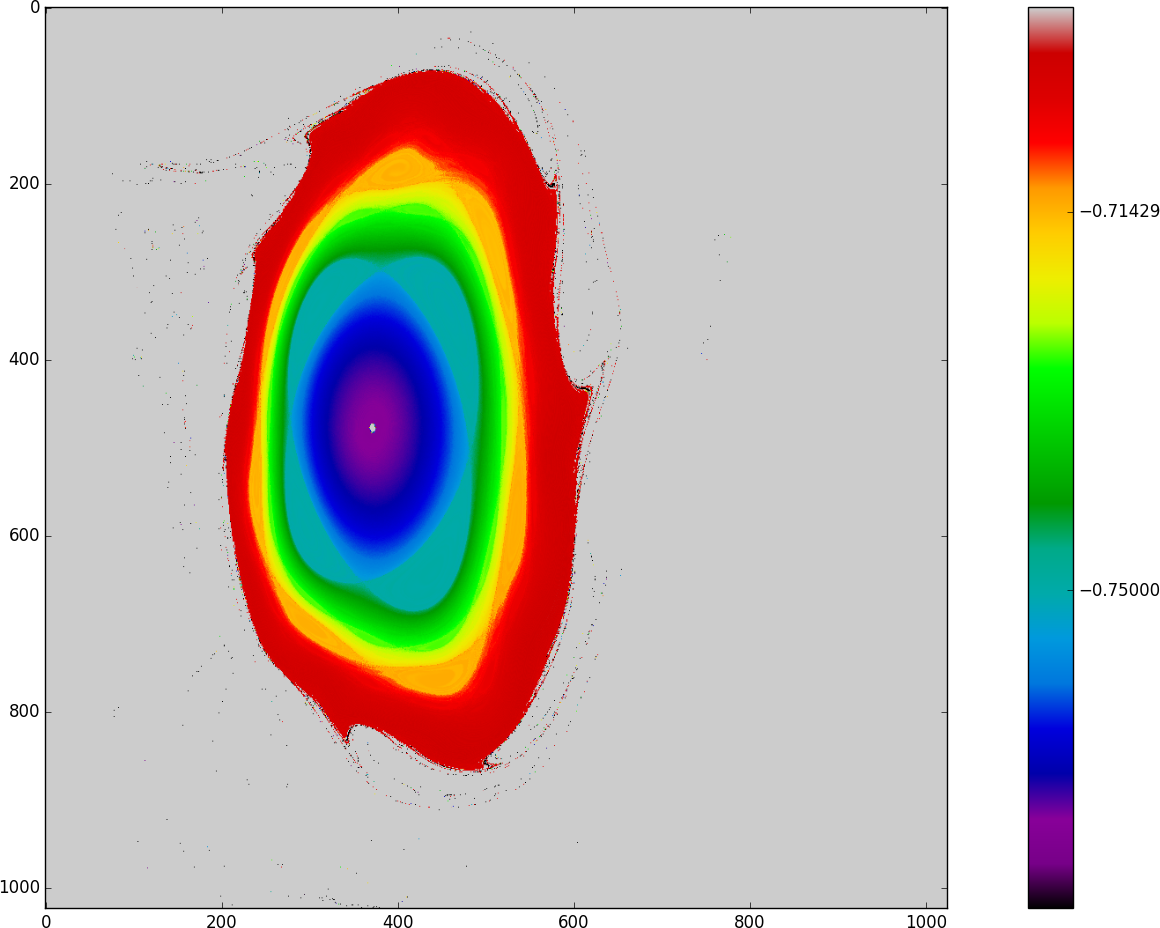
\includegraphics[width=\linewidth]{Figures/Rings_Papertwist_twist1_82_steps32k.png}
  \caption{Winding numbers of the field lines of a cross-section through the torus. The vertical axis was scaled since the winding number is almost constant. The vector field used is "Papertwist1-82". The image is $1024\times 1024$ pixels, with $32768$ points per field line.}\label{fig:82-32k}
\endminipage\hfill
\minipage{0.32\textwidth}
  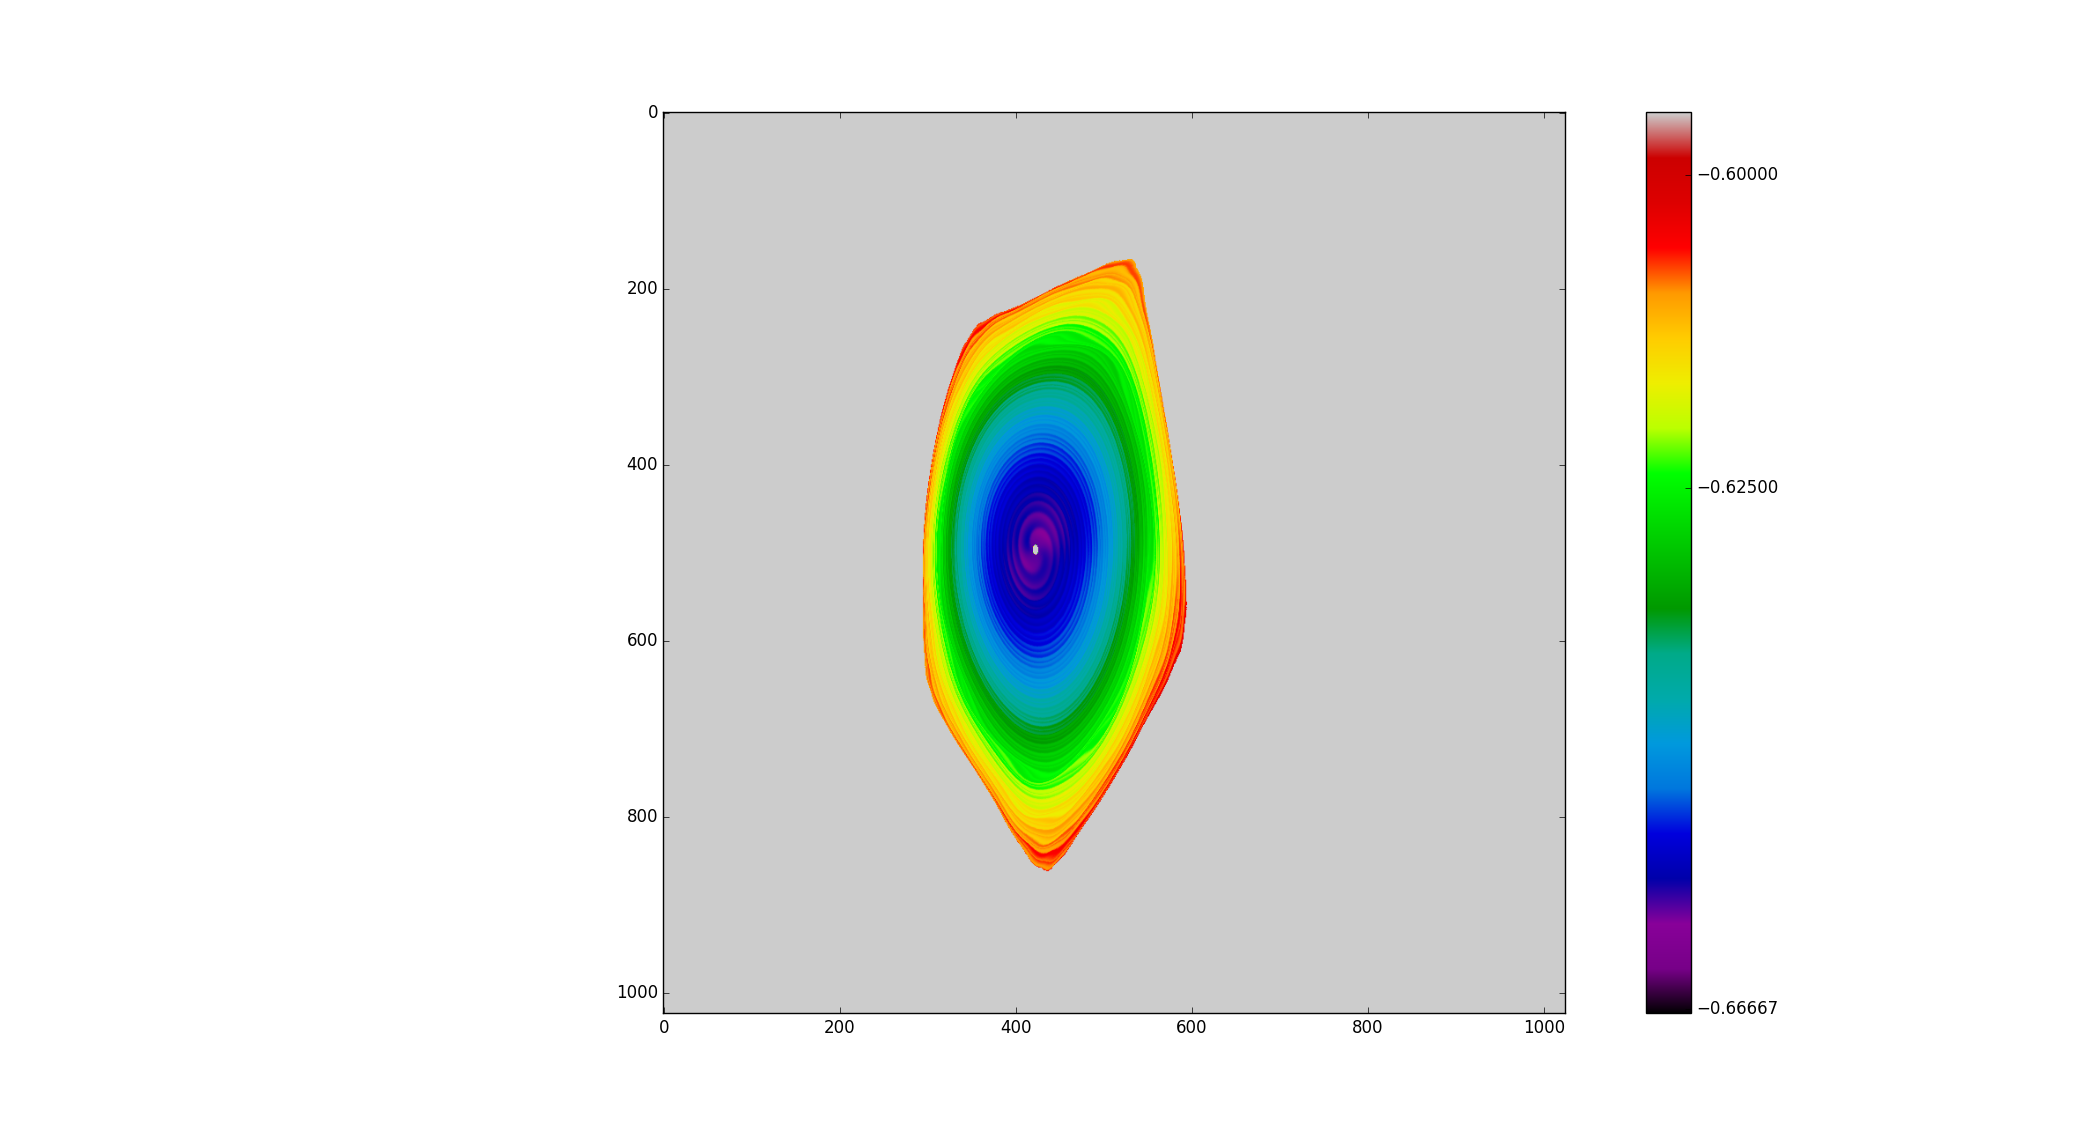
\includegraphics[width=\linewidth]{Figures/Rings_Papertwist_twist1_125_steps8k.png}
  \caption{Winding numbers of the field lines of a cross-section through the torus. The vertical axis was scaled since the winding number is almost constant. The vector field used is "Papertwist1-125". The image is $1024\times 1024$ pixels, with $8196$ points per field line.}\label{fig:125-8k}
\endminipage\hfill
\minipage{0.32\textwidth}%
  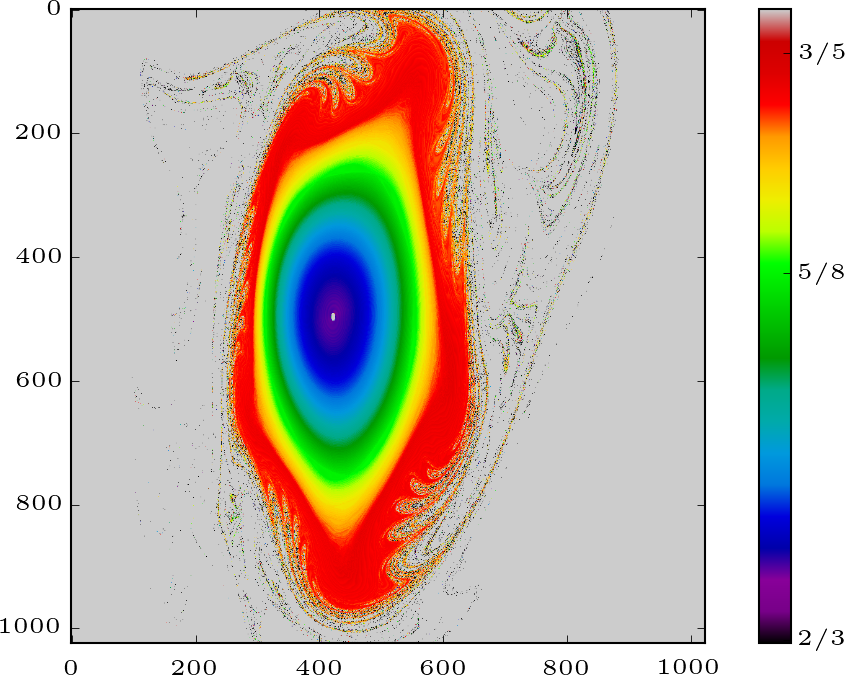
\includegraphics[width=\linewidth]{Figures/Rings_Papertwist_twist1_125_steps32k.png}
  \caption{Winding numbers of the field lines of a cross-section through the torus. The vertical axis was scaled since the winding number is almost constant. The vector field used is "Papertwist1-125". The image is $1024\times 1024$ pixels, with $32768$ points per field line.}\label{fig:125-32k}
\endminipage
\end{figure}

In order to make a good image we had to restrict the data in two ways. We firstly changed the colour scale (as mentioned in the caption above) to ensure that the changes in the nearly-constant winding number are visible. Secondly we have discarded (masked) all the points with low total length of the field line, reasoning that the winding numbers of short field lines can be wildly inaccurate. For completeness we include a plot of the length of the field lines and the unmasked (but still colour-clipped) data in figure \ref{fig:125-32k} below.

\begin{figure}[!htb]
\minipage{0.48\textwidth}
  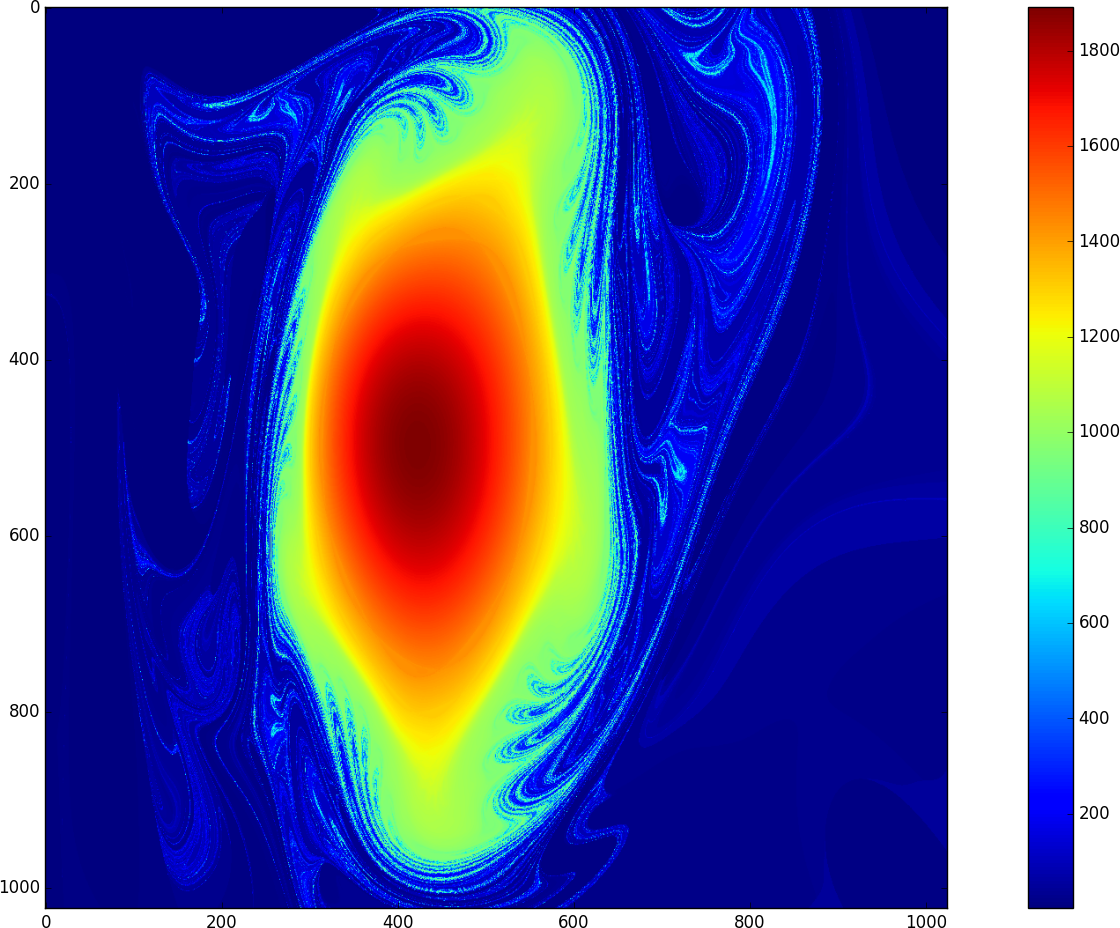
\includegraphics[width=\linewidth]{Figures/Rings_Papertwist_twist1_125_lengths_steps32k.png}
  \caption{Lengths of the field lines of a cross-section through the torus. The vector field used is "Papertwist1-125". The image is $1024\times 1024$ pixels, with $32768$ points per field line.}\label{fig:125-lengths}
\endminipage\hfill
\minipage{0.48\textwidth}
  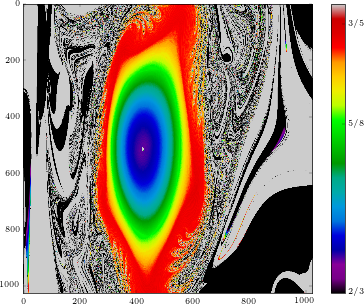
\includegraphics[width=\linewidth]{Figures/Rings_Papertwist_twist1_125_nomask_steps32k.png}
  \caption{Unmasked winding numbers of the field lines of a cross-section through the torus. The vector field used is "Papertwist1-125". The image is $1024\times 1024$ pixels, with $32768$ points per field line.}\label{fig:125-unmasked}
\endminipage
\end{figure}



\subsection{Speed and scaling}
We have recorded the runtime of the code for the dataset "Shafranov Rot3 ampl 0,05 Animation50", generating and analysing datasets as in figures \ref{fig:82-32k}-\ref{fig:125-32k}. For the first set of timing data we fixed the image size at $1024\times 1024$ pixels (field lines) and varied the number of steps per field line. After that we fixed the number of steps per field line (at $32768$) and varied the number of pixels (field lines) in an image.\\

\textbf{Insert graphs on speed here!}\\

We compared the performance of our program with an older simulation which also computed winding numbers for plasma field lines that was in use before our code was available. The older code simulated a $1\times 1100$ array of field lines with $4000-16000$ steps per line, and took approximately $36$ hours for this simulation. Comparing this with our own results we conclude that our program is faster by approximately a factor of $3.5\cdot 10^6$.\\

Lastly we used the NVIDIA visual profiler to see how much memory our code was using while active. While generating a $1024\times 1024$ dataset with $32768$ steps per field line the program was using $6513$ MiB while in use, whereas running the code with identical parameters except for halving the number of steps per line (to $16384$) the program was using $3441$ MiB.


\section{Discussion}
{\bf Algoritmekeuzes \textrightarrow betere keuzes, sign flip in center: niet meer nodig?, stitching issues: niet meer nodig?, aannames over geometrie, dynamische stapgrootte, fringes door fouten $(\alpha,\beta)$-afronding.}\\

\subsection{Optimization}
Because the numerical integration is the only inherently sequential part of the algorithm, we made the choice to minimize calculations during this part of the algorithm. Profiling of the code shows however that it is heavily memory bandwidth bound. This suggest more calculations can be done during integration to improve use of the other computational resources during this part of the algorithm.\\

\subsection{Numerical errors}
There are two features in the results that merit further discussion. Firstly we remark that near the center of each of the cross-sections the winding numbers behave oddly (the small white dots in the center of figures \ref{fig:82-32k}-\ref{fig:125-32k}). Closer inspection of the unmasked data reveals that there is a sign flip in the winding number of the field lines here, which shows up as white due to the colour scale. We expect that this supposed sign flip is an error in the code, possibly caused by the change in coordinate systems. Since our transformation of Cartesian coordinates to Toroidal coordinates is based on the line data it is possible that this coordinate change becomes inaccurate for small tori. In particular we determine a radius of and normal to a circle around the origin of a field line, and assume that this circle lies inside the torus on which the field line lies. If this circle intersects a cross-section of the torus near the edge of the cross-section all results based on the toroidal coordinate system will contain a small error (whereas it would be perfect if they intersect in the centre of the cross section). If this intersection instead happens outside the torus we can safely say that all winding numbers computed in the toroidal coordinate system are useless. Since in practice the tori on which the field lines lie may be highly elliptical (instead of perfectly circular) the only way to completely avoid this error may be through more thorough analysis of these surfaces.\\

Secondly it is interesting to consider the differences between figure \ref{fig:125-8k} and figure \ref{fig:125-32k}, in particular the apparent shapes near the center of the cross section. In figure \ref{fig:125-8k} we clearly see shapes with twofold rotational symmetry around the white center, which have disappeard in figure \ref{fig:125-32k}. We suspect that these patterns in the winding numbers may be due to the finite length of the simulated field lines. Since (as mentioned above) the surfaces on which our field lines lie are not perfect tori but rather are slightly elliptical, there are sections of field line where the local winding number is not equal to the global (average) winding number along a line. Therefore after a finite number of data points the average of our simulated line may disagree with the true winding number (corresponding to an infinitely long line). This problem is made far worse by the fact that our toroidal coordinate system is not optimized for correcting this eccentricity, which explains why these features are most prominent at the center of the cross section. A possible solution might be to use a more sophisticated method to extract the global winding number from the local data than the (weighed) average that is currently in place, although it should be noted that most of these methods are hard to parallellize and will therefore significantly slow down the algorithm.\\

We would furthermore like to remark that, as always when numerically integrating a vector field, there is a tradeoff between small step size (and low truncation error in the numberical method) and large step size (and low total number of steps for fixed length, so a low cumulative rounding error). In our code we fix the step size inversely proportional to the average length of the magnetic field that is supplied. Therefore actual step, with a length of our step size times the local magnitude of the magnetic field, is on average constant between different input fields. A possible improvement on this would be to dynamically scale the step size at each integration step, ensuring that the total steps taken are of very similar length. However these additional computations will slow down the algorithm.\\

\subsection{Speed and scaling}
We note that the memory usage agrees well with our theoretical predictions, where we consider that we store (for the $32768$ steps per line):
\begin{itemize}
\item The vector field, $256\times256\times256$ 'Float4' objects ($16$ Byte each), for a total of $256$ MiB.
\item The line data itself, $64\times 64$ lines (this part of the code is serialized so not all lines need to be stored at the same time) times $32768$ 'Float4' points per line, for a total of $2048$ MiB.
\item One array to compute and store the normal vectors to the tori of interest, which needs to be of the same size as the line data array, so $2048$ MiB total.
\item Two scalar fields to compute and store the toroidal and poloidal windings of $64\times 64\times 32768$ Floats, which equals $512$ MiB per field or $1024$ MiB total.
\item One scalar field to compute and store the length of the vector fields, for $512$ MiB total.
\item One scalar field to compute and store the middle radius of the tori, for $512$ MiB total.
\end{itemize}
In total this adds up to $6400$ MiB, which is in good agreement with the observed $6513$ MiB. To find the theoretical memory use for the simulation with $16384$ steps per field line we repeat the calculation above and find a total of $3328$ MiB in theory, which agrees well with the $3441$ MiB experimentally observed. In both cases we are using $113$ MiB more than was predicted in theory, which we attribute to general overhead.\\

Secondly we observe that, as was predicted, the runtime of our code is highly linear in both the number of pixels/field lines and the number of steps per field line, with an offset of \textbf{insert offset here}. We conclude that this is the amount of time that it takes to load the vector field to the memory on the graphics card and allocate all relevant arrays, and that the complexity of the algorithm is as predicted.

\section{Suggestions for future work}

\subsection{Interpolation}
Better algorithms exist for interpolation, most notably cubic interpolation and interpolation schemes which preserve the zero divergence of the magnetic field\cite{McNally01052011}. It is possible that these algorithms could further reduce numerical artefacts. %TODO Which artefacts.
Notably, efficient and open source implementations in CUDA of cubic interpolation exist.\cite{Ruijters01012012}

\subsection{Integration}
As mentioned the code was shown to be largely memory access bound. Implementation of a multi-step method such as Adams-Bashforth could reduce the number of texture fetches per step, while maintaining a high order.\\
Also worth mentioning is that the RK4 integration method uses no special properties of the magentic field, such as the divergencelessness or the Hamiltonian description. It might for example be possible to exploit the knowledge that the system is Hamiltonian by implementing a symplectic method.

\subsection{Optimization}
We remarked before that profiling the code revealed that the algorithm is both memory bound and memory access bound. A possible optimization would be to increase the computational load during the integration of the magnetic field, for example pre-calculating some of the properties required later.



\bibliographystyle{plain}
\bibliography{introduction}
\end{document}
